\subsection{Auckland}

Comencemos por describir la ruta generada:
Se han realizado 22 saltos hasta alcanzar el destino solicitado, de los cuales en el $72 \% $ de los mismos aproximadamente, hemos obtenido respuestas del tipo $TIME\_EXCEEDED$, determinando así que el largo de nuestra ruta es de 16 saltos, y que del resto de los valores del $TTL$ no hemos obtenido respuesta alguna. Como también se puede ver en la figura \ref{mapa-auckland}, y en el cuadro \ref{tabla-auckland}, durante el trayecto se realizaron 3 saltos intercontinentales. Por otra parte, el método de Cimbala nos ha detectado en un principio todo número positivo como outlier, pero al sacar los 0s sólo ha detectado aquellos que se muestran en el cuadro ya mencionado.

\begin{table}[!htbp]
\centering
\caption{My caption}
\label{tabla-auckland}
\begin{tabular}{|c|c|c|c|}
\hline
\textbf{TTL} & \textbf{IP}    & \textbf{COUNTRY} & \textbf{OUTLIERS} \\ \hline
1   & 10.0.2.2        & Undefined     &               \\ \hline
6   & 200.89.161.133  & Argentina     & {[}outlier{]} \\ \hline
7   & 200.89.165.5    & Argentina     &               \\ \hline
8   & 200.89.165.250  & Argentina     &               \\ \hline
9   & 190.216.88.33   & Argentina     &               \\ \hline
10  & 67.17.94.249    & Australia     & {[}outlier{]} \\ \hline
13  & 4.68.127.54     & United States &               \\ \hline
14  & 129.250.4.250   & United States &               \\ \hline
15  & 129.250.2.219   & United States & {[}outlier{]} \\ \hline
16  & 129.250.7.69    & United States & {[}outlier{]} \\ \hline
17  & 129.250.3.123   & United States &               \\ \hline
18  & 204.1.253.166   & United States &               \\ \hline
19  & 202.158.194.172 & Australia     & {[}outlier{]} \\ \hline
20  & 182.255.119.139 & Australia     &               \\ \hline
21  & 210.7.39.251    & New Zealand   &               \\ \hline
22  & 210.7.39.178    & New Zealand   & {[}outlier{]} \\ \hline
\end{tabular}
\end{table}

\newpage

\begin{figure}[!htbp]
  \centering
    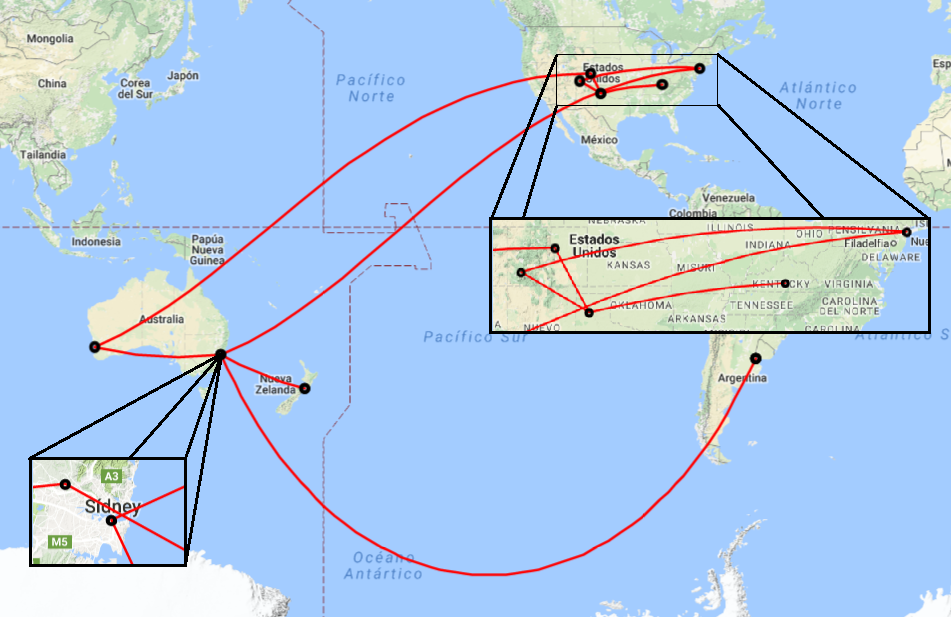
\includegraphics[scale=0.6]{imagenes/auckland-graficos/mapa-auckland.png}
  \caption{auckland- RTT hops}
  \label{mapa-auckland}
\end{figure}

En este contexto, nos disponemos a realizar un análisis más profundo de nuestros resultados. Podemos observar entonces, que de los 3 saltos intercontinentales, Cimbala identifica correctamente todos, salvo el primer salto de Australia a EEUU, y a su vez, indica 4 saltos como outliers que no son intercontinentales realmente. En resumen, si contamos todo outlier como salto intercontinental, obtenemos en esta muestra:

\begin{itemize}
	\item $18 \% $ de falsos positivos aprox.
	\item $4 \%$ de falsos negativos aprox.
	\item $78 \%$ de resultados acertados aprox.
\end{itemize}

Realizando un análisis parecido al realizado con Oxford, podemos observar en la figura \ref{fig:8} que la mayoría de los puntos se concentran apenas encima del 0.4, y cualquier otro punto que no respete esta línea, es considerado outlier. Nuevamente observamos que si solo tomamos los puntos por encima de este valor, nos quedan los saltos intercontinentales. Esta vez, podríamos atribuir el falso negativo a que, como se observa en la figura \ref{fig:7} , el rtt correspondiente al salto es francamente muy bajo, tomando un valor por debajo de los 5 ms.

\begin{figure}[!htbp]
  \centering
    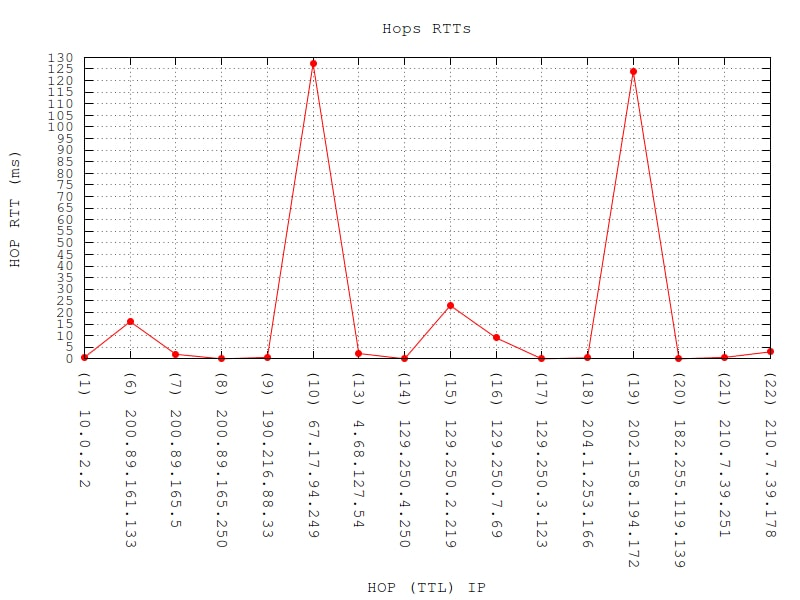
\includegraphics[scale=0.6]{imagenes/auckland-graficos/traceroute-auckland.jpg}
  \caption{auckland- RTT hops}
  \label{fig:7}
\end{figure}

\begin{figure}[!htbp]
  \centering
    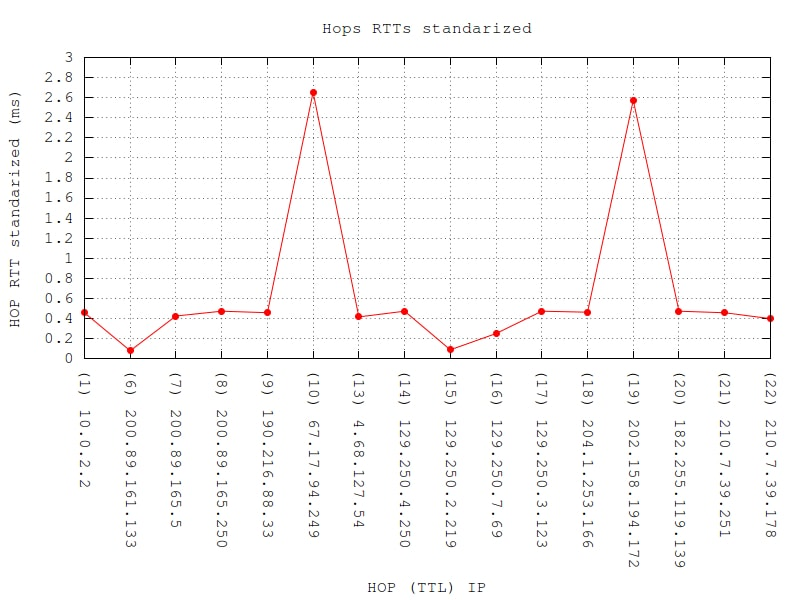
\includegraphics[scale=0.6]{imagenes/auckland-graficos/traceroute-auckland-standarized.jpg}
  \caption{auckland- RTT hops standarized}
  \label{fig:8}
\end{figure}


Resumiendo, si consideramos solo los valores que en la figura \ref{fig:8} que están por encima del punto de acumulaciónPONGANME UN BUEN NOMBRE, pasamos a obtener un $96\%$ de aciertos, siendo el $4\%$ restante un caso muy curioso.

